\chapter{Thin strip graphs}
\label{chap:thinDef}

\todo{Introduction of the chapter.}

\todo{Explain Breu's characterization of strip graphs}

$c$-strip graphs are unit disk graphs such that the centers of the disks belong to
$\{(x,y) : -\infty < x < \infty, 0 \leq y \leq c\}$. The class is denoted by SG($c$). We
have SG(0) = UIG and SG($\infty$) = UDG. \cite{hayashiThinStripGraphs2017}

\begin{defn}
  Thin strip graphs are defined as TSG $= \bigcap_{c > 0}$ SG($c$).
\end{defn}

\begin{remark}
  SG($0$) $\neq$ TSG. We can construct a $K_{1,3}$ such that we have 3 vertices with the coordinates
  $(1,0)$, $(0,0)$, $(1,0)$ and a last one $(0,\varepsilon)$ with $\varepsilon > 0$ and arbitrarily small
  as seen in Figure \ref{fig:thinK13}.
\end{remark}

% Figure about the K_1,3 construction
\begin{figure}
\centering

\begin{scaletikzpicturetowidth}{\textwidth}
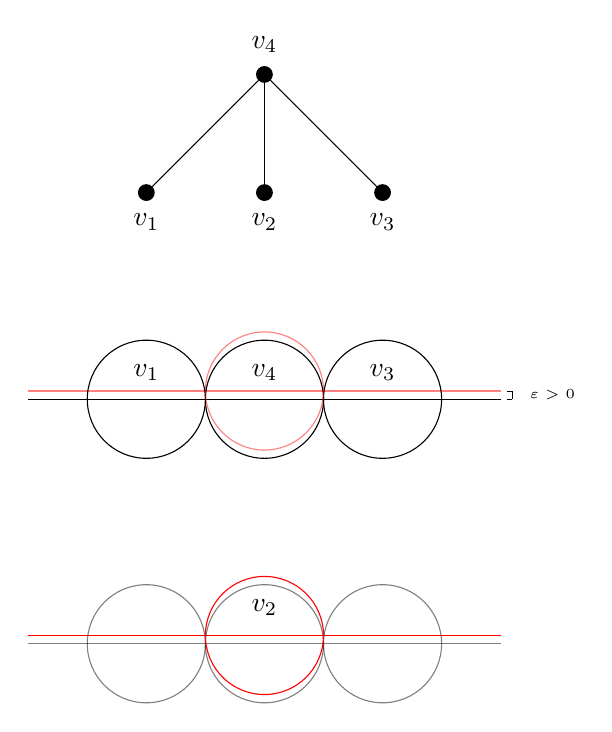
\begin{tikzpicture}[scale=1.5]

\draw (-2,0) -- (2,0);
\draw[red ,opacity = 0.5] (-2,0.07) -- (2,0.07);
\draw  (-1,0) circle [radius=0.5];
\draw[color=black] (-1,0.2265) node {$v_1$};
\draw  (0,0) circle [radius=0.5];
\draw[color=black] (0,0.2265) node {$v_4$};
\draw  (1,0) circle [radius=0.5];
\draw[color=black] (1,0.2265) node {$v_3$};

\draw[red, opacity = 0.5] (0,0.07) circle [radius=0.5];
\draw[color=black] (2.4386,0.0367) node {\tiny $\varepsilon > 0$};

% lines to describe distance (epsilon)
\draw[very thin] (2.1,0.07) -- (2.1,0);
\draw[very thin] (2.05,0.07) -- (2.1,0.07);
\draw[very thin] (2.05,0) -- (2.1,0);

\draw[opacity = 0.5] (-2,-2.07) -- (2,-2.07);
\draw[red] (-2,-2) -- (2,-2);
\draw[opacity = 0.5]  (0,-2.07) circle [radius=0.5];
\draw[opacity = 0.5]  (1,-2.07) circle [radius=0.5];
\draw[opacity = 0.5]  (-1,-2.07) circle [radius=0.5];
\draw[red] (0,-2) circle [radius=0.5];
\draw[color=black] (0,-1.765) node {$v_2$};

\node[draw,circle,inner sep=2pt,fill,label distance=1cm] (v1) at (0,2.75) {};
\draw[color=black] (0,3) node {$v_4$};
\node[draw,circle,inner sep=2pt,fill,label distance=1cm] (v3) at (0,1.75) {};
\draw[color=black] (0,1.5) node {$v_2$};
\node[draw,circle,inner sep=2pt,fill,label distance=1cm] (v2) at (-1,1.75) {};
\draw[color=black] (1,1.5) node {$v_3$};
\node[draw,circle,inner sep=2pt,fill,label distance=1cm] (v4) at (1,1.75) {};
\draw[color=black] (-1,1.5) node {$v_1$};
\draw  (v1) edge (v2);
\draw  (v1) edge (v3);
\draw  (v1) edge (v4);
\end{tikzpicture}
\end{scaletikzpicturetowidth}
\caption{A construction of $K_{1,3}$ with a disk realization, being this graph a TSG.}
\label{fig:thinK13}
\end{figure}

\begin{theorem}[Hayashi et al. \cite{hayashiThinStripGraphs2017}]
  There is no constant $t$ such that SG($t$) = TSG.
\end{theorem}

Since this class is newly defined we have to characterize it. For this purpose,
some relations have been found between this class and interval graphs.

\subsection{Interval graphs}

\begin{theorem}[Hayashi et al. \cite{hayashiThinStripGraphs2017}]
  MUIG $\subsetneq$ TSG.
\end{theorem}

We can define a new class of graphs: unfettered unit interval graphs. These graphs
are unit interval graphs where if two intersections touch, we can decide whether
they intersect or not. We denote this class UUIG.

\begin{theorem}[Hayashi et al. \cite{hayashiThinStripGraphs2017}]
  TSG $\subsetneq$ UUIG.
\end{theorem}


\section{Characterization of thin strip graphs}

One of the main goals of this thesis is to characterize TSG. by forbidden induced subgraphs. To approach this, we will see how many induced forbidden subgraphs are also forbidden for TSG. We have described the familes of forbidden induced subgraphs for MUIG in section \ref{sec:muig} and one of these familes has been proven to be a forbidden induced subgraph for TSG:

\begin{theorem}[Hayashi et al. \cite{hayashiThinStripGraphs2017}]
  $\mathcal{R}$ is a forbidden induced subgraph family of TSG.
\end{theorem}

\begin{figure}
\centering

\begin{scaletikzpicturetowidth}{\textwidth}
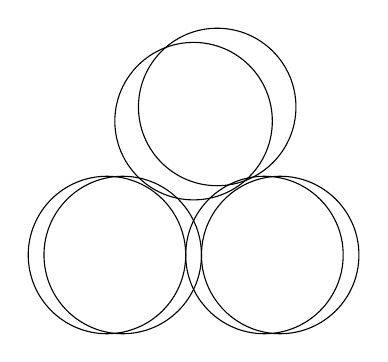
\begin{tikzpicture}[scale=2]

%\draw  (0.1,0) circle [radius=0.5];
%\draw  (0,0) circle [radius=0.5];
%\draw  (-0.3,-0.95) circle [radius=0.5];
%\draw  (0.3,-0.7) circle [radius=0.5];
%\draw  (-0.7,-1) circle [radius=0.5];
%\draw  (0.9,-0.7) circle [radius=0.5];

% line
\draw  (0,0) circle [radius=0.5];
\draw  (0.1,0) circle [radius=0.5];
\draw  (1,0) circle [radius=0.5];
\draw  (1.1,0) circle [radius=0.5];

%upper
\draw  (0.55,0.85) circle [radius=0.5];
\draw  (0.7,0.94) circle [radius=0.5];


\end{tikzpicture}
\end{scaletikzpicturetowidth}

\caption{A construction of $F$ with a unit disk realization.}
\label{fig:fUDG}
\end{figure}


With the properties presented in this chapter, we can begin to state our first hypothesis:

\begin{hyp}
  $F \in (\text{UDG}\cap\text{UUIG}) \setminus \text{TSG}$.
\end{hyp}

\begin{claim}
 $F \in (\text{UDG}\cap\text{UUIG})$
\end{claim}

\begin{proof}
  We can see that $F \in$ UDG because we can have a unit disk realization (Figure \ref{fig:fUDG}) and also has a level structure $L = \{K_2, K_3, K_1\}$.
\end{proof}

\begin{theorem}
$F \notin$ TSG.
\end{theorem}

\proof{
We define $\overrightarrow{G}$ as the complement oriented digraph of $G$ where $\overrightarrow{G} = (V,\overrightarrow{E})$ being $\overrightarrow{E}$ an orientation of $\overline{E}$.

The orientation of $\overrightarrow{E}$ is based in the partial order on the $x$-coordinate of the vertices such that:

$$ \overrightarrow{E} = \{uv: \phi(u)_x < \phi(v)_x \forall u,v \in V\}$$

\todo[inline]{Now we have to check either there is a POSSIBLE partial order of $\overrightarrow{E}$ or there is not a dangerous cycle with more than 2 nodes of $ \overrightarrow{G}$ in the cycle... (to explain in rdv).}
}

\section{Recognition}

The recognition of this class of graphs is stated by Breu in his thesis \todo{explain everything about dangerous cycles and
complement oriented graphs in Breu's paper}.
